% $Id: introduction.tex 1784 2012-04-27 23:29:31Z nicolas.cardozo $
% !TEX root = main.tex

\chapter{Tool: Debugger}
\label{cha:debugger}

In this chapter, we present the design and implementation of the debugger tool.
The debugger is a key component of the proposed framework, as it allows 
developers to interact with the RL program during execution, inspect the 
internal state of the agent, and modify its behavior in real-time.

As it is shown in the figure below, the debugger features an interface where 
the top left pane displays the user's code that is intended to be debugged. 
In the top right pane, the variables currently loaded by the program and their 
corresponding values can be observed. This pane also serves as an interface for 
the user to modify the values of variables in real-time. Additionally, the user 
can select variables of interest to monitor during execution.

At the top, the current execution point of the program is displayed, which 
can be paused, continued, or restarted. Finally, the bottom section shows 
the interaction graph of the variables during the program's execution, which 
updates in real-time.

\begin{figure}[h]
    \centering
    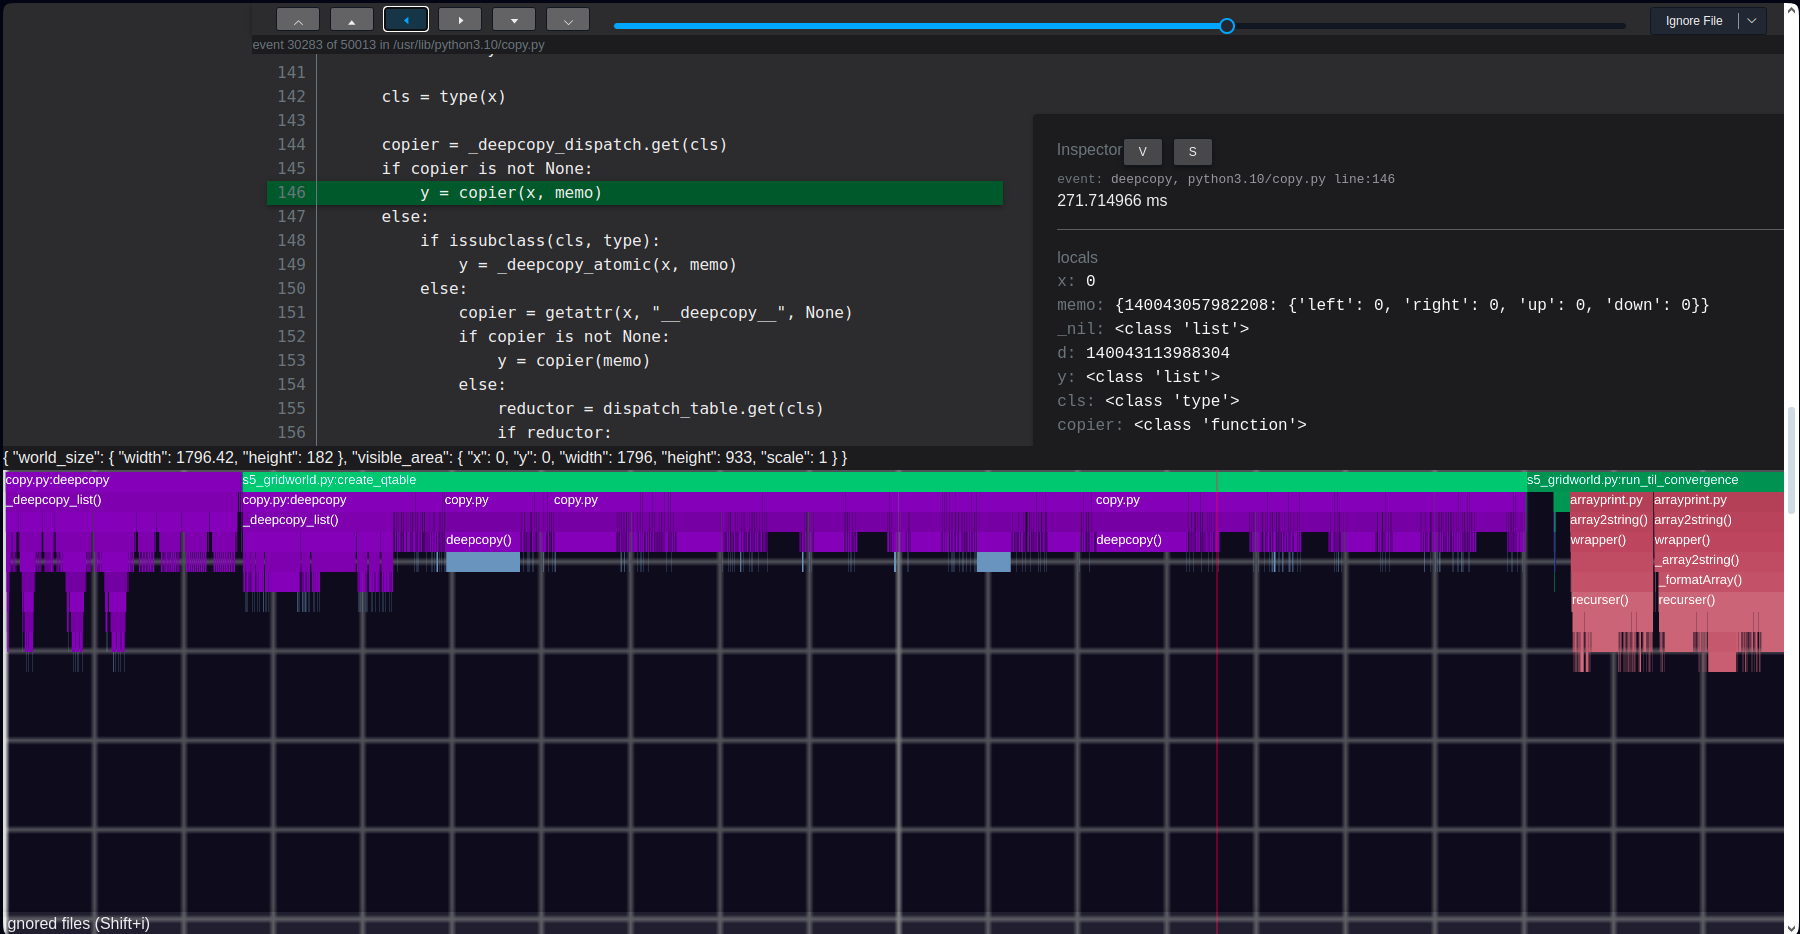
\includegraphics[width=1\textwidth]{figures/tool.png}
    \caption{Debugger tool}
    \label{fig:debugger}
\end{figure}


\endinput